% !TEX root = ./pkMain.tex
\mode*


\begin{frame}
\frametitle{Kompartiment Modelle: Abstraktion}

\note<1>{
\begin{itemize}
\item
Zeichne: Pictogramm Mensch: Spritze: Injektion $\Rightarrow$ xy Grafik mit Konzentrationsverlauf.
\item
Es gibt Formeln die Kurven ergeben. (z.B. $C = (Dosis * Gewicht)^{t}$)
\item
Formel kann nicht jede Form haben da: z.B. Konzentration f\"allt ab, Abfall abh\"angig von Konzentration etc.
\item
Was abl\"auft bei der graphischen Darstellung kann als Formel ausgedr\"uckt werden.
\end{itemize}
}
\end{frame}

%: PK Studie

\frame{ \begin{exampleblock}{Ablauf einer PK Studie:}
     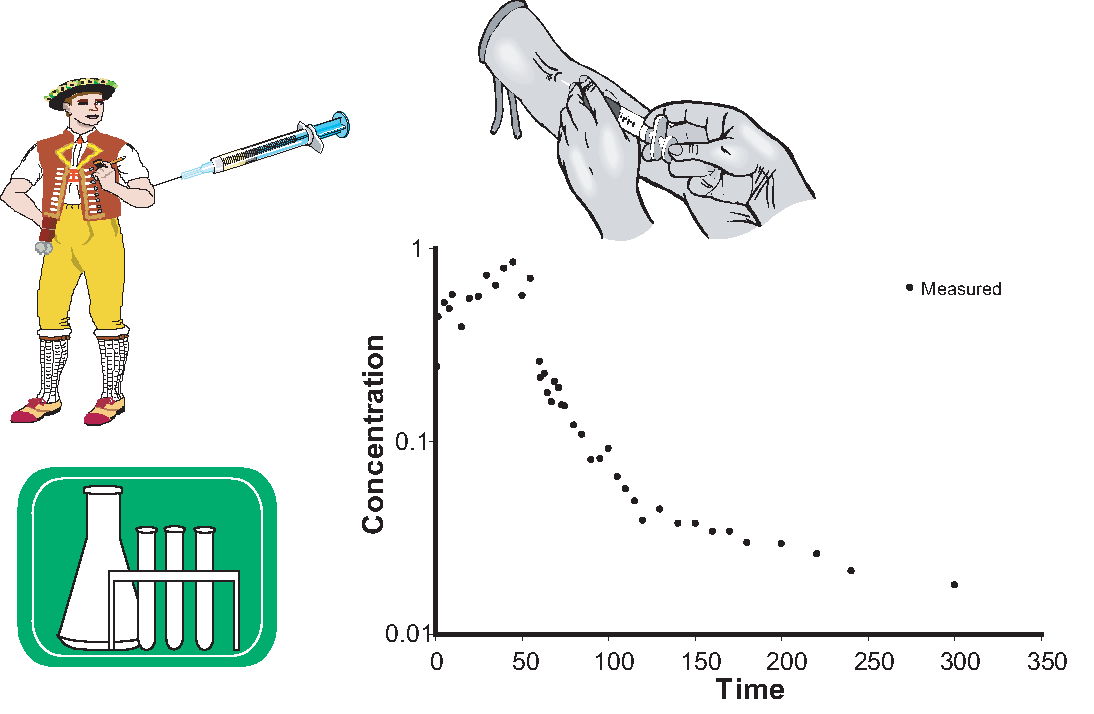
\includegraphics[clip=true,width=\textwidth]{PKStudy.pdf}
\end{exampleblock}
\note<1>{
\begin{itemize}
\item
Ablauf zeigen: Menschen, mehrere Individuen
\item
In die Grafik zeichnen.
\end{itemize}}
}


\frame{
\begin{alertblock}{Herleitung von PK Modellen basiert auf:}
    \begin{itemize}
        \item Bekanntem Input (z.B. meist eine konstante Infusion) und gemessenen Konzentrationen
        \item Nichtlinearer Regression zu Bestimmung der Modellparameter: $V_1$,$V_2$,$V_3$,$Cl_1$,$Cl_2$,$Cl_3$
    \end{itemize}
    \begin{center}
        \href{run:Fitsimulation.xls}{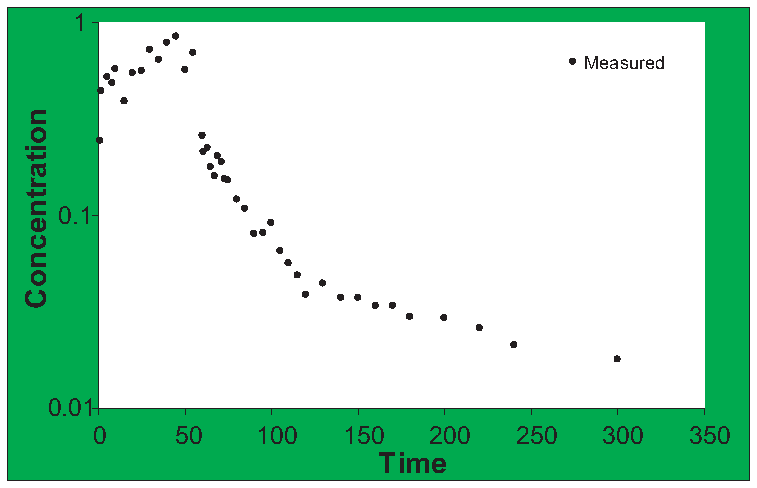
\includegraphics[width=8cm]{ForFitSim.pdf}}
    \end{center}
\end{alertblock}
\note<1>{ Beachte den Text im Manuskript.\\
Bei der Simulation die verschiedenen Parameter ver�ndern und auf die
Ver�nderung der Kurve aufmerksam machen.\\
Die Sch�ler sollen die Kurve durch die Datenpunkte im Manuskript
einzeichnen.}
}


\begin{frame}
\frametitle{Individualisieren!}
\begin{itemize}[<+->]
\item Es m�ssen viele \enquote{verschiedene} Patientengruppen untersucht werden. (m/f, dick/d�nn, alt/jung)
\item Die Unterschiede zwischen den einzelnen untersuchten Patienten m�ssen gesucht werden
\item F�r jeden zuk�nftgen Patienten k�nnen dann  mit dem Modell die passenden Parameter berechnet werden. (siehe Eingabe in TCI)
\end{itemize}
\note<1>{}
\infina
\end{frame}

